
\subsubsection{$m_h$ and $\sigma_{Zh}$}
\label{sec:higgs:sigmazh}
The signal processes are $\ee\to Zh$, $Z\to l^+l^-$ or $q\bar{q}$ and 
$h\to$anything. Thanks to the known four momenta of initial states, 
the four momentum of final state $h$ can be reconstructed 
as the recoil against the four momentum of $Z$, which is directly
measured from its decay products $l^+l^-$ or $q\bar{q}$. 
The mass of $h$ ($m_X$) can therefore be reconstructed as
\beq
m_X^2=s+m_Z^2-2E_Z\sqrt{s},
\eeq{eqn:recoilmass}
where $m_Z$ and $E_Z$ are measured mass and energy of $Z$
respectively. The signal events can hence be tagged without looking
at the decay products of $h$. This technique is traditionally called
{\it recoil mass} technique, and the two types of signal processes 
($Z\to l^+l^-$ and $Z\to q\bar{q}$) are called
leptonic recoil and hadronic recoil channels. The recoil mass technique
makes possible the measurement of the inclusive cross section of $\ee\to Zh$ ($\sigma_{Zh}$),
that plays a unique role in the determination of the absolute values of
Higgs couplings as explained in Sec.~\ref{sec:physics}.
Meanwhile, the Higgs mass ($m_h$) can be straightforwardly determined by 
the $m_X$ spectrum. The detailed analyses for leptonic recoil channels
$\mu^+\mu^-h$ and $e^+e^-h$ and for hadronic recoil channel $q\bar{q}h$
can be found respectively in references~\cite{Yan:2016xyx} and 
~\cite{Tomita:2015,Thomson:2015jda,Miyamoto:2013zva}. 
For simplicity only the analysis for $\mu^+\mu^-h$ channel is illustrated in detail here.

The event pre-selection in $\mu^+\mu^-h$ channel starts with requiring at least 
two isolated muons with opposite charges and invariant mass ($m_{ll}$) consistent 
with $Z$ mass ($m_{ll}\in[50,130]$ GeV). 
It is well possible that one or two muons in such a candidate 
muon pair are actually from Higgs decay, for instance from 
$h\to ZZ^*/WW^*/\tau^+\tau^-\to \mu^+\mu^-+others$. To minimize the possibility of
this case, or to maximize the possibility that the candidate muon pair is 
indeed from the primary $Z$ decay, a strategy is taken:
when there are more than one such candidate muon pairs,
the pair which minimizes following $\chi^2$ 
\beq
\chi^2=(\frac{m_{ll}-M_Z}{\sigma_Z})^2+(\frac{m_{X}-M_h}{\sigma_h})^2
\eeq{eqn:chi2forleptonpair}
is identified as from the primary $Z$ decay. Here $M_Z$ is 91.2 GeV,
$M_h$ is 125 GeV, $\sigma_Z$ and $\sigma_h$ are resolutions for 
$Z$ mass and recoil mass reconstructions. 
After the pre-selection, the remaining background events are dominated by
leptonic and semi-leptonic decays of $\ee\to ZZ$, leptonic decay of $\ee\to WW$, 
and leptonic decay of $\ee\to \gamma Z$. 

In the final-selection, cuts $p_T^{ll}>10$ GeV and $|\cos\theta_{mis}|<0.98$,
where $p_T^{ll}$ is the transverse momentum of muon pair and $\theta_{mis}$
is the polar angle of missing four momentum, are applied to suppress
$\gamma Z$ background events. $E_{vis}>10$ GeV,
where $E_{vis}$ is the visible energy other than the muon pair,
and $m_{ll}\in[73,120]$ GeV
are applied to suppress $WW$ background events. 
$ZZ$ as well as $WW$ and $\gamma Z$ background events are
further suppressed by a dedicated BDT cut 
which is trained using distributions of polar angle of each muon,
angle between two muons, and polar angle of the muon pair. After a final cut that requires
$m_X\in[110, 155]$ GeV, the remained signal and background events are 
shown in the $m_X$ spectrum in Fig.~\ref{fig:RecoilMassLep250} 
for the $Z\to\mu^+\mu^-$ channel, where the signal peak is clearly seen.
The overall signal efficiency is 88\%, with an
average signal over background ratio of 1/1.3.

The number of signal events and its statistical uncertainty are obtained by 
fitting $m_X$ spectrum with signal component modeled by a kernel function
and background component modeled by a third order polynomial, 
shown in Fig.~\ref{fig:RecoilMassLep250}. As shown by the green histogram in Fig.~\ref{fig:RecoilMassLep250},
the signal spectrum has a 
considerable non-Gaussian tail in the high mass end, which is due to
the overestimate of effective $\sqrt{s^\prime}$ in $\ee\to Zh$ reaction 
when beamstrahlung and ISR effects are included, recall Eqn.~\ref{eqn:recoilmass}.
It's worth noting that these effects become so significant at $\sqrt{s}=500$ GeV,
as shown in Fig.~\ref{fig:RecoilMassLep500},
that the measurement uncertainty could be underestimated by a factor of 2
if the effects are not properly included in the simulation. 

\begin{figure}
\begin{center}
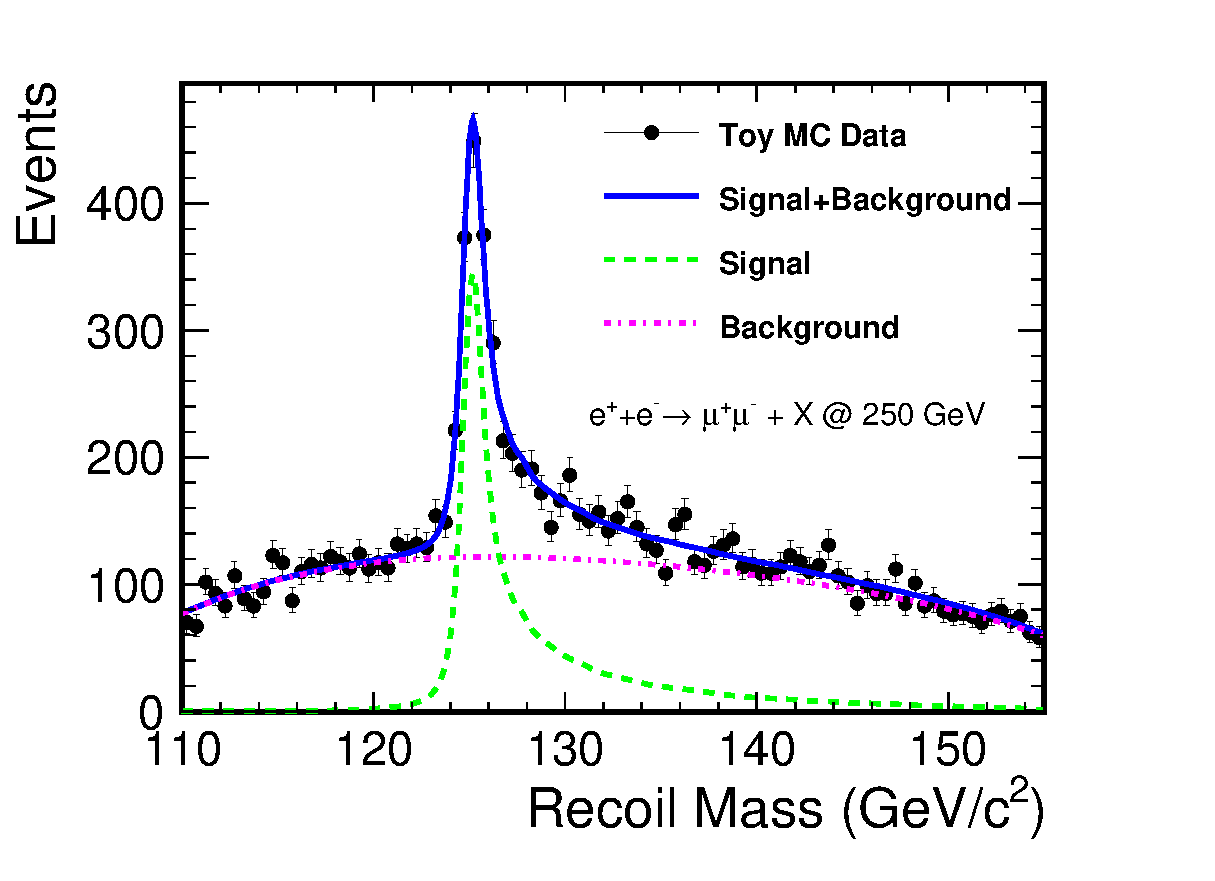
\includegraphics[width=0.85\hsize]{chapters/figures/RecoilMassLep250.eps}
\end{center}
  \caption{Recoil mass spectrum against
 $Z\to\mu^+\mu^-$ for signal $e^+e^-\to Zh$ and SM background 
  at 250 GeV \cite{Yan:2016xyx}.}
  \label{fig:RecoilMassLep250}
\end{figure}

\begin{figure}
\begin{center}
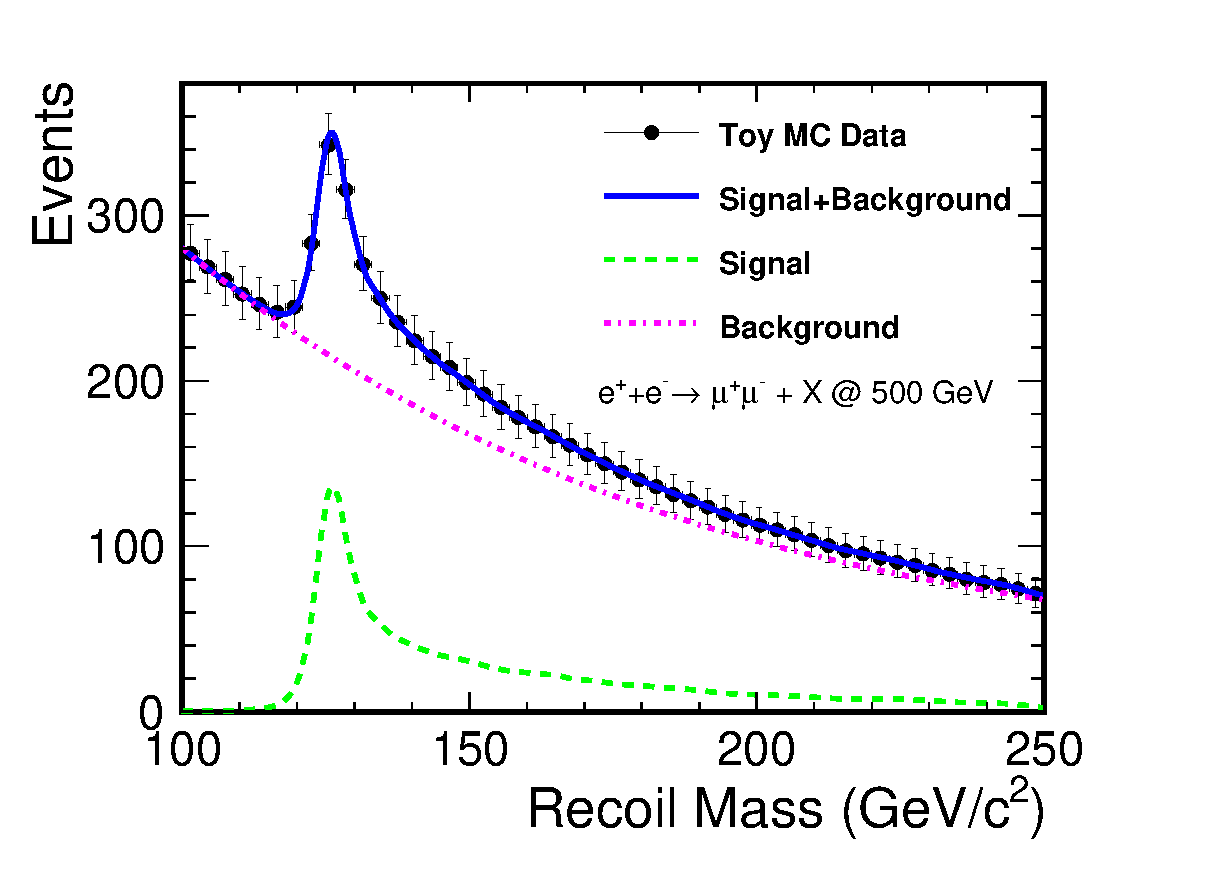
\includegraphics[width=0.85\hsize]{chapters/figures/RecoilMassLep500.eps}
\end{center}
  \caption{Recoil mass spectrum against
 $Z\to\mu^+\mu^-$ for signal $e^+e^-\to Zh$ and SM background 
  at 500 GeV \cite{Yan:2016xyx}.}
  \label{fig:RecoilMassLep500}
\end{figure}

For $e^-_Le^+_R$, the estimate of relative 
uncertainty on $\sigma_{Zh}$ measurement ($\delta\sigma_{Zh}$) 
is 2.5\% for the leptonic
recoil channel, where the contribution from $e^+e^-h$ channel is
slightly smaller than $\mu^+\mu^-h$ channel due to the higher 
electron bremsstrahlung. For $e^-_Re^+_L$, $\delta\sigma_{Zh}$
is estimated to be 2.9\%. By combining the hadronic recoil channel,
$\delta\sigma_{Zh}$  is estimated to be 2.0\% for both $e^-_Le^+_R$
and $e^-_Re^+_L$, as shown in~\ref{tab:higgserrors}. 
The enabled measurement of left-right asymmetry 
for $\sigma_{Zh}$ plays a very important role in the EFT fit as
explained in Sec.~\ref{sec:physics}. 
The Higgs mass $m_h$ is also measured from the fit shown
in Fig.~\ref{fig:RecoilMassLep250}. The estimate of $m_h$ uncertainty 
is 14 MeV for ILC250, with the dominant contribution 
from $\mu^+\mu^-h$ channel. 
The uncertainty in the Higgs boson mass ($\delta m_h$) does play a role 
as a source of systematic error for predictions of Higgs boson couplings. 
In most cases, $\Delta m_h\sim 100$ MeV 
would be already sufficient, but this is not true
for $h\to ZZ^*$ or $h\to WW^*$. 
It has been pointed out in  \cite{Lepage:2014fla} that 
\beq
\delta_W =6.9\cdot\delta m_h,~~~~\delta_Z =7.7\cdot \delta m_h,
\eeq{eqn:MassH}
where $\delta_W$ and $\delta_Z$ are the 
relative errors for $g(hWW)$ and $g(hZZ)$ respectively. 
At ILC250, the 14 MeV accuracy for Higgs boson mass results in 
systematic errors of 0.1\% for $\delta_W$ and
$\delta_Z$.


\begin{table}[htb]
\centering
\begin{tabular}{l|c|c|c|c|c|c|c|c}
\hline
${h\to }$ & bb & cc & gg & $\tau\tau$ & $\mathrm{WW^{*}}$ & 
$ZZ^{*}$ & $\gamma\gamma$ & $\gamma Z$ \\
\hline
eff. [\%] & 88.25 & 88.35 & 87.98 & 88.43 & 88.33 & 88.52 & 88.21 & 87.64 \\
\hline
\end{tabular}
\caption{The efficiencies of the major SM Higgs decay modes,
after all the event selection cuts, shown here for the case 
of the $\mathrm{\mu^{+}\mu^{-}h}$
channel and $e_{L}^{-}e_{R}^{+}$ at $\sqrt{s}$=250 GeV~\cite{Yan:2016xyx}.
The uncertainties due to finite MC statistics on these values are below 0.14\%.}
\label{tab:recoilmass}
\end{table}

As pointed out in the very beginning of this analysis, the key idea which enables
the inclusive $\sigma_{Zh}$ measurement is that the signal is tagged
independently of Higgs decay modes. Hence it is crucial to examine whether all
the pre-selection and final-selection cuts satisfy this criterion. This can be verified 
by checking the signal efficiency for each individual Higgs decay mode
and evaluating the efficiency uniformity among all the decay modes.
Table~\ref{tab:recoilmass} lists the efficiencies of major SM Higgs decay modes 
after all cuts in the $\mu^+\mu^-h$ channel. It is seen that there is no
discrepancy in efficiencies of SM decay modes beyond 1\%. 
This is not a surprise because the analysis strategies and selection cuts
are carefully designed to make it so. The cut $E_{vis}>10$ GeV may
deserve a few more words, since it apparently suppresses the 
$h\to invisible$ mode. The strategy behind is that $\sigma_{Zh}$ can be
measured as 
\beq
\sigma_{Zh}=\sigma_{Zh}^{vis}+\sigma_{Zh}^{inv},
\eeq{eqn:sigmazh}
where $\sigma_{Zh}^{vis}$ is the total cross section for all $h\to visible$
modes, which is measured here, and $\sigma_{Zh}^{inv}$ is the cross section
for $h\to invisible$ mode, which can be measured separately, described in
Sec.~\ref{sec:higgs:invisible}. A detailed and quantitative analysis taking into 
account the possibility of existing BSM decay modes is performed in~\cite{Yan:2016xyx}.
It concludes that the relative bias on $\sigma_{Zh}$,
induced by the Higgs decay modes dependence, can be
controlled at below 0.1\% (0.2\%) for the $\mu^+\mu^-h$ ($e^+e^-h$) channel,
which is much smaller than the
expected statistical uncertainty even at the full ILC250.

In the hadronic recoil channel, a more complicated strategy is applied in order to
keep the analysis still decay modes independent. In stead of the simple categorization
into visible and invisible modes in leptonic channel, the signal events in hadronic channel
are categorized according to number of taus, number of leptons, and number of jets
in the final state. In principle as long as the categories are inclusive we can design and 
optimize the selection cuts category by category. The studies in~\cite{Tomita:2015} show
that by varying the SM decay branching ratios by $\pm 5\%$ (absolute) in each decay mode,
the bias on measured $\sigma_{Zh}$ is at most around 0.5\% relatively.  
More efforts would be needed in future to further reduce the bias to a much lower level
in particular even under assumption that there would be other unknown exotic decay modes.
At higher $\sqrt{s}$, the hadronic recoil analysis generally becomes less challenging, because
the two jets from primary $Z$ are more boosted hence are easier to 
be identified from the Higgs decay products, as studied in~\cite{Thomson:2015jda,Miyamoto:2013zva}
for $\sqrt{s}=350$ and 500 GeV.

\subsubsection{$\sigma_{\nu\nu h}$ and $\sigma_{eeh}$}
\label{subsubsec:higgs:nunuee}

The second leading Higgs production process, 
$\ee\to\nu\bar{\nu}h$ via $W$-fusion, provides a direct measurement
for $hWW$ coupling. It plays a crucial role in the global fit based on $\kappa$ formalism,
and still helps improve the global fit results based on EFT formalism even though 
the cross section is not very large at $\sqrt{s}=250$ GeV, 
$\sigma_{\nu\nu h}=$ 14 fb for $e^-_Le^+_R$. 
The signal channel used is 
$e^+e^-\to\nu\bar{\nu}h,~h\to b\bar{b}$, in which direct observable is
$\sigma_{\nu\nu h}\cdot BR_{bb}$. Together with $BR_{bb}$ measurement
by $Zh$ process, $\sigma_{\nu\nu h}$ is then measured.
The analysis is briefly described here, and more details can be found 
in~\cite{Durig:2014lfa,Tian:2017}. 

\begin{figure}
%\begin{center}
\begin{tabular}[c]{c}
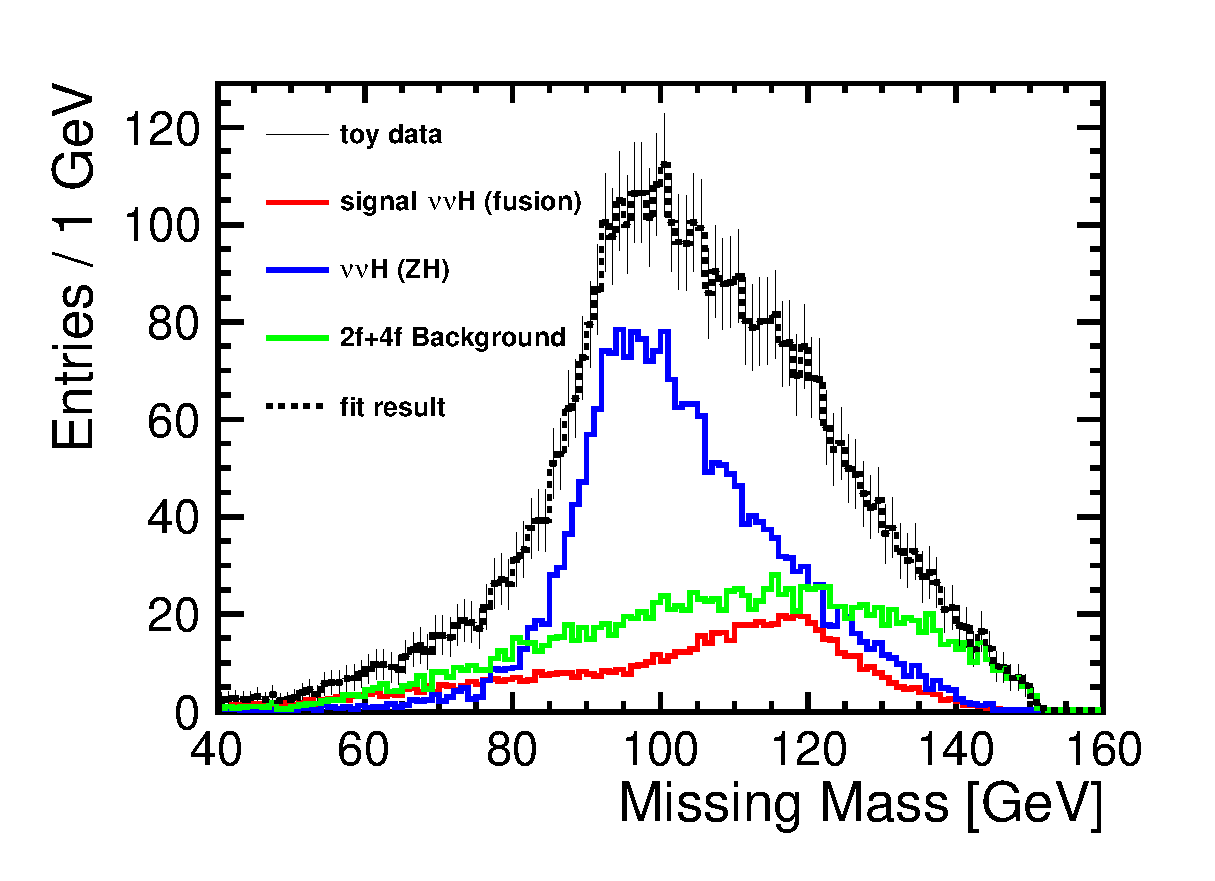
\includegraphics[width=0.85\hsize]{chapters/figures/vvH_MissingMass250.eps} \\
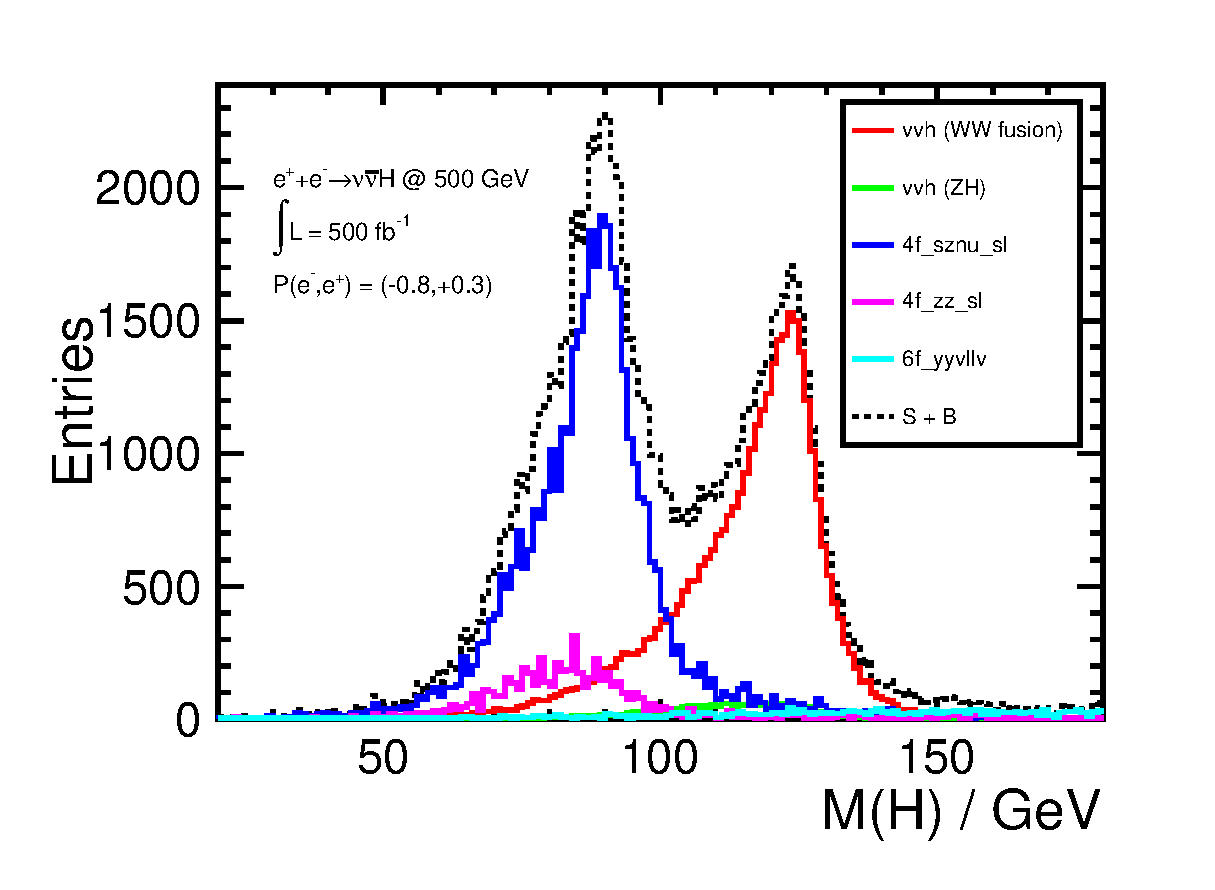
\includegraphics[width=0.85\hsize]{chapters/figures/vvH_MassH500.eps}
\end{tabular}
%\end{center}
  \caption{Missing mass spectrum (upper) and Higgs mass spectrum (lower) 
  for the signal $e^+e^-\to\nu\bar\nu h, h\to b \bar{b}$ and the SM background 
  at 250 GeV and 500 GeV respectively \cite{Durig:2014lfa,Tian:2017}.}
  \label{fig:vvHbb}
\end{figure}

\begin{figure*}[htb]
\begin{center}
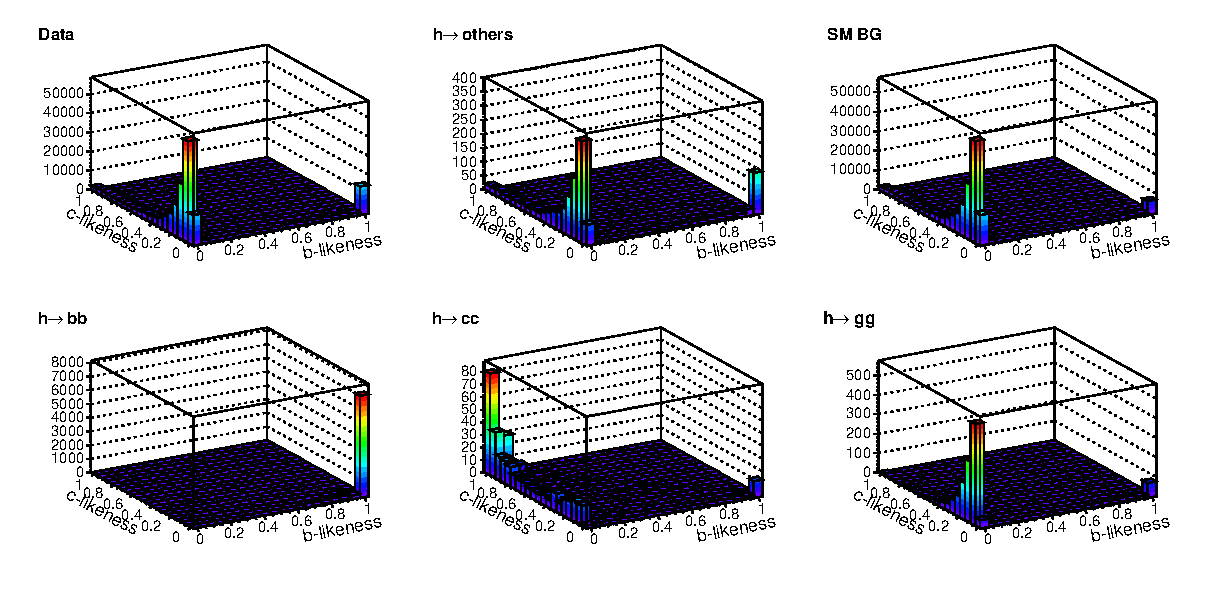
\includegraphics[width=0.85\hsize]{chapters/figures/qqh_bbccgg_template_250.eps}
\end{center}
  \caption{Template of b-likeliness versus c-likeness for signal $h\to b\bar{b}/c\bar{c}/gg$
  (bottom left/middle/right) events,
and for $h\to others$ / SM background (top middle/right) events, and distribution for 
all the events (top left), in $Z\to qq$ channel normalized to 250 fb$^{-1}$. The b-likeness
is defined as a combined function of the two b-tags (say $x_1$ and $x_2$) 
of the two jets from $h$ candidate: $\mathrm{b-likeness} = \frac{x_1x_2}{x_1x_2+(1-x_1)(1-x_2)}$.
The c-likeness is defined in a similar way.}
  \label{fig:qqHbbccgg250}
\end{figure*}

The signal final states consist of two b-jets and two missing neutrinos.
The pre-selection starts with vetoing events with one or more isolated 
leptons. Then jet-clustering and flavor tagging are performed with expected number of
jets equals 2. The two jets are required that in each jet there are at least 6
reconstructed particles and $Y_{3\to2}<0.1$, where $Y_{3\to 2}$ is the 
jet distance value from 3 jets to 2 jets step defined by Durham algorithm. The 
b-tagging of the two jets are required to be $btag1>0.8$ and $btag2>0.2$.
The di-jet invariant mass is required to be $m_{bb}\in[110,150]$ GeV.
The missing mass is required to be larger than 20 GeV.
After the pre-selection, the remaining dominant background events are
from $\gamma Z$ ($Z\to b\bar{b}$), $\nu\bar{\nu}Z$ ($Z\to b\bar{b}$) 
and $Zh$ ($Z\to\nu\bar{\nu}$, $h\to b\bar{b}$).

In the final-selection, $\gamma Z$ and $\nu\bar{\nu}Z$ background 
events are further highly suppressed by a BDT cut, which is trained 
using input variables di-jet mass, polar angle of di-jet, angle between
two jets, and $Y_{2\to1}$. The remained signal and background events
are plotted in the missing mass spectrum, shown in Fig.~\ref{fig:vvHbb} (upper).
The signal efficiency is 36\% and the average signal over background ratio is around 1/4.
The most dominant background events turn out to come from $Zh$ ($Z\to\nu\bar{\nu}$) and 
have significant overlap with signal events in the missing mass spectrum.
This is because the invariant mass of $\nu\bar{\nu}$ of signal events
can not be far away from $M_Z$, limited by available phase space at $\sqrt{s}=250$ GeV.
Therefore it is necessary to fit simultaneously $\sigma_{\nu\nu h}\cdot BR_{bb}$
and $\sigma_{Zh}\cdot BR_{bb}$. Note a useful constraint can be added into the fit
that $\sigma_{Zh}\cdot BR_{bb}$ is also measured 
using $Z\to l^+l^-$ and $Z\to q\bar{q}$ channels. 
As a result, the estimate of relative uncertainty on $\sigma_{\nu\nu h}\cdot BR_{bb}$
is 8.1\%, shown in Table~\ref{tab:higgserrors}, 
and the correlation between $\sigma_{\nu\nu h}\cdot BR_{bb}$ and
$\sigma_{Zh}\cdot BR_{bb}$ is -34\%.

The left-handed beam polarization does help significantly the $\sigma_{\nu\nu h}$
measurement here, simply because it enhances the cross section by a factor of 2.34.
The $\sigma_{\nu\nu h}$ can be measured much better at $\sqrt{s}=500$ GeV, 
shown in~\ref{fig:vvHbb} (lower), thanks
to a fact of 10 increase on cross section and much easier separation with $Zh$ ($Z\to\nu\bar{\nu}$).

The third leading Higgs production process, $\ee\to e^+e^- h$ via $Z$-fusion, is not easy to measure
due to its very small cross section at $\sqrt{s}=250$ GeV, $\sigma_{eeh}=0.7$ fb. 
A full simulation analysis is performed and 
suggests that this process is already discoverable at $\sqrt{s}=250$ GeV with 2 ab$^{-1}$ and
$\sigma_{eeh}$ can be measured with a significance of 9$\sigma$~\cite{Ogawa:2018}. 
At $\sqrt{s}=500$ GeV, the significance will be significantly improved to 60$\sigma$.

\subsubsection{$\mathrm{BR}(h\to b\bar{b}/c\bar{c}/gg)$}
The capabilities of precise measurements for $\mathrm{BR}(h\to c\bar{c}/gg)$ 
mark down another unique advantage of a lepton collider, enabled by:
clear separation between b-jet, c-jet and light quark/gluon-jet thanks to the
excellent flavor tagging performance introduce in Sec.~\ref{sec:software};
more importantly the democracy about cross sections between Higgs processes and
other SM background processes induced by electroweak interactions.
$\mathrm{BR}(h\to b\bar{b}/c\bar{c})$ offer important measurements of 
Yukawa couplings between Higgs and third/second generation quarks. 
$\mathrm{BR}(h\to gg)$ offers direct measurement of $hgg$ coupling 
using, complementary to that at the LHC. These measurements are performed
using the leading Higgs production process $\ee\to Zh$. All the major $Z$ decay
channels $Z\to l^+l^-$, $Z\to\nu\bar{\nu}$ and $Z\to q\bar{q}$ are used in the analyses,
see details in~\cite{Ono:2013sea}. Following illustrated is the analysis procedure 
for $Z\to q\bar{q}$ channel. 

The signal final states consist of four jets, common for $h\to b\bar{b}/c\bar{c}/gg$. 
In the pre-selection, all the particles
in each event are first clustered into four jets using Durham algorithm. The
four jets are paired into two di-jet pairs, $j_1j_2$ and $j_3j_4$, 
as for respectively $Z$ and $h$ candidates by minimizing the $\chi^2$ defined as 
$$\chi^2=(\frac{m_{j_1j_2}-M_Z}{\sigma_Z})^2+(\frac{m_{j_3j_4}-M_h}{\sigma_h})^2,$$
where $m_{j_1j_2}$ ($m_{j_3j_4}$) is the invariant mass of $j_1j_2$ ($j_3j_4$),
and $\sigma_Z$ ($=4.7$ GeV) and $\sigma_h$ ($=4.4$ GeV) are the widths
of invariant mass spectra of $Z$ and $h$ respectively determined using MC truth information. 
A cut $\chi^2<10$ is applied. In the final-selection, to suppress the leptonic or 
semi-leptonic background events, the number of
charged particles in each jet is required to be $> 4$. To suppress the $q\bar{q}$
background events, the jet clustering parameter $Y_{4\to3}$ 
is required to be consistent with 4-jet characteristic, that $\log Y_{4\to 3}>-2.7$.
In addition two cuts are applied on the event thrust and thrust angle,
that $\mathrm{thrust}<0.9$ and $|\cos\theta_{\mathrm{thrust}}|<0.9$. The remaining
background events are dominated by $q\bar{q}q\bar{q}$, mainly from hadronic decays of $WW$ and $ZZ$. 
A cut on the angle between $j_3$ and $j_4$ is applied, $105^\circ<\theta_{j_3j_4}<160^\circ$.
A kinematic fitting, using four-momentum conservation constraints plus 
$m_{j_1j_2}-m_{j_3j_4=M_Z-M_h}$ constraint, is performed. And two cuts are
applied on the fitted $Z$ and $h$ masses, 
that $m_{j_1j_2}\in[80,100]$ GeV and $m_{j_3j_4}-M_h\in[-15,10]$ GeV. As a final cut,
a multivariate likelihood is derived and required to be $\mathrm{Likelihood}>0.375$.
After all the cuts, the signal efficiency is 26\%, with an average $S/B$ ratio of around 1/10, 
including all events of $h\to b\bar{b}/c\bar{c}/gg$ (note the $S/B$ ratio for $h\to b\bar{b}$ events
is much higher). 

A template fit is then performed to extract the numbers of signal events $h\to b\bar{b}$,
$h\to c\bar{c}$ and $h\to gg$ respectively, 
for which it is crucial that the different signal events are distinguishable with themselves 
as well as with background events. 
The templates are constructed as 3-D histograms using
3 variables, namely b-likeness, c-likeness and bc-likeness defined for the two jets 
$j_3$ and $j_4$ (as from $h$ candidate). Five templates are made using separated MC samples:
signal $h\to b\bar{b}$, $h\to c\bar{c}$, $h\to gg$, SM background and $h\to\mathrm{others}$ background. 
The projected 2-D templates for b-likeness versus c-likeness are shown in Fig.~\ref{fig:qqHbbccgg250}, 
each of which has been normalized to an integrated luminosity of 250 fb$^{-1}$.
It demonstrates that the three types of signal events can indeed be clearly distinguished
with themselves and with background events, thanks to
the excellent flavor tagging performance and good signal over background ratio.

We just used $Z\to q\bar{q}$ channel to illustrate the analysis, it is worth commenting that 
$Z\to\nu\bar{\nu}$ channel is as powerful as $Z\to q\bar{q}$ channel despite its branching ratio
is a factor of 3 smaller. This is largely due to the factor that the signal and background 
discrimination in $Z\to q\bar{q}$  channel is much degraded by performance of 
the realistic jet clustering and jet pairing algorithms at now, 
as a result of which the S/B ratio in $Z\to q\bar{q}$ channel is a factor of 5
lower than that in $Z\to\nu\bar{\nu}$ channel. From the perspective of a better jet clustering
or jet pairing algorithm in future, the analysis in $Z\to q\bar{q}$ channel can be 
significantly improved.

By combining $Z\to q\bar{q}/\nu\bar{\nu}/l^+l^-$ channels, 
the estimates of statistical uncertainties for $\sigma_{Zh}\cdot BR_{bb}$,
$\sigma_{Zh}\cdot BR_{cc}$ and $\sigma_{Zh}\cdot BR_{gg}$ are respectively
1.3\%, 8.3\% and 7.0\%, shown in Table~\ref{tab:higgserrors}.

\subsubsection{$\mathrm{BR}(h\to WW^*/ZZ^*)$}
The measurements of branching ratios of $h\to WW^*/ZZ^*$ play an important role
in the global fit as the Higgs total width is determined by
$$\Gamma_h=\frac{\Gamma_{WW}}{BR_{WW}}=\frac{\Gamma_{ZZ}}{BR_{ZZ}}.$$
Depending on how each $W/Z$ decays and how Higgs is produced, there
are quite many signal channels that can be used. The analysis strategies as well as
the signal background discrimination also vary quite a lot channel by channel.
For $Zh$ production and $h\to WW^*$, 
the signal channels are listed in Table~\ref{tab:ZhWWchannels}, where the channels
with marks are studied based on full simulation and enter the combined estimate of 
statistical uncertainty. The details of event selections can be found in~\cite{Ono:2012,Barklow:2017,Liao:2017}.
One of the dominant background processes in all channels is $e^+e^-\to W^+W^-$, suppression of which 
can be helped by the right-handed beam polarizations.
Due to the multiple jets in the signal final states, the analysis could also benefit significantly 
from an improved jet clustering algorithm in future.
The estimate of statistical uncertainties for $\sigma_{Zh}\cdot BR_{WW}$ is
4.6\%, shown in Table~\ref{tab:higgserrors}. It's worth noting from Table~\ref{tab:ZhWWchannels}
that there are still many more channels which yet to be employed in full simulation in future 
to improve the $\sigma_{Zh}\cdot BR_{WW}$ measurement, in particular the fully hadronic channel 
 $Z\to q\bar{q}$ and $WW^*\to qqqq$ that has the largest branch ratio.

\begin{table}
\begin{center}
\begin{tabular} {lcccccc}
$h\to$ / $Z\to$  & $l^+l^-$ &  $\nu\bar{\nu}$ & $q\bar{q}$ \\
\hline
$WW^*\to qqqq$        & 3.0\%$^{**}$    & 9.0\%$^{*}$   & 31\% \\
$WW^*\to qql\nu$      & 2.0\%    & 5.8\%    & 20\%$^{*}$ \\
$WW^*\to l\nu l\nu$   & 0.3\%    & 1.0\%    & 3.3\%
\end{tabular}
\caption{Signal channels in $e^+e^-\to Zh,~h\to WW^*$ and their branching ratios. 
The entries marked with * or ** are currently studied by full simulation and enter the combined result. 
The entry marked with ** is based on CEPC studies.}
\label{tab:ZhWWchannels}
\end{center}
\end{table}


\begin{figure}
\begin{center}
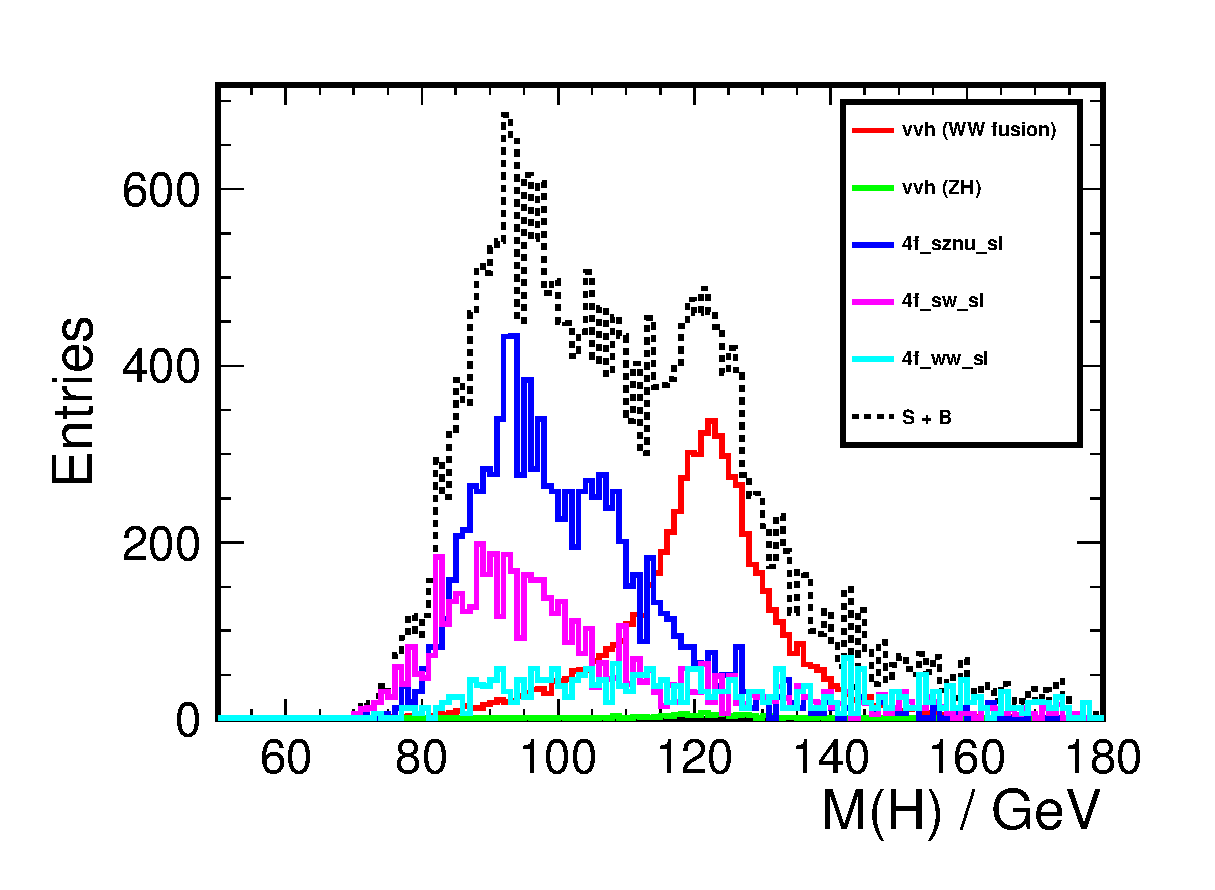
\includegraphics[width=0.85\hsize]{chapters/figures/vvH_WW4j500_MassH.eps}
\end{center}
  \caption{Higgs mass spectrum for the signal $e^+e^-\to\nu\bar\nu h, h\to WW^{*}\to qqqq$
  and the SM background events, normalized to 500 fb$^{-1}$
  at 500 GeV \cite{Durig:2014lfa}.}
  \label{fig:vvHWW500}
\end{figure}

\begin{figure}
\begin{center}
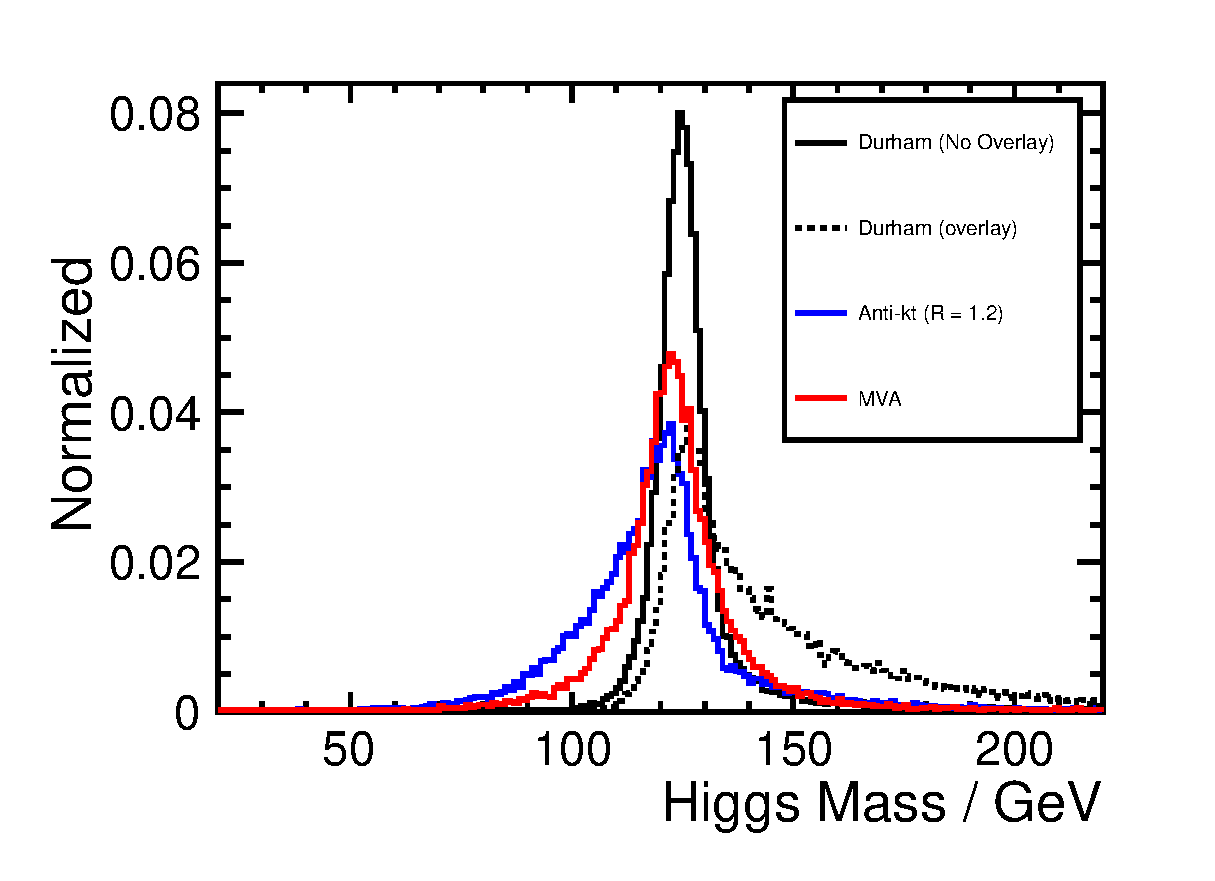
\includegraphics[width=0.85\hsize]{chapters/figures/vvH_WW4j500_Overlay.eps}
\end{center}
  \caption{Higgs mass spectrum for the signal $e^+e^-\to\nu\bar\nu h, h\to WW^{*}\to qqqq$
   in different cases of overlay: no overlay (solid black) 
  illustrating the performance of perfect overlay removal; without overlay and without
  applying any removal algorithm (dashed black); overlay removal with traditional 
  exclusive jet clustering algorithm, anti-$k_T$ here (blue); overlay removal with a new
  method based on MVA, optimized for this particular signal channel (red). The histograms 
  are normalized to 500 fb$^{-1}$ at $\sqrt{s}=$500 GeV \cite{Durig:2014lfa}.}
  \label{fig:vvHWW500ovl}
\end{figure}

At $\sqrt{s}=500$ GeV, the $BR(h\to WW^*)$ measurement can also be improved significantly by including 
Higgs production via $W$-fusion. Two signal channels $e^+e^-\to\nu\bar{\nu}h$, $h\to WW^*\to qqqq / qql\nu$
have been studied based on full simulation. As an illustration, 
the remained signal and background events in $WW^*\to qqqq$ channel
after all cuts are plotted in Fig.~\ref{fig:vvHWW500} in the reconstructed $h$ mass spectra. The signal peak
can be clearly observed with the dominant background from $\nu\bar{\nu}h$ ($h\to others$), 
$\nu\bar{\nu}Z$ and $W^+W^-$. The average S/B ratio is around $1/1.6$ in the $M(h)\in(114,142)$ GeV 
region. The estimate of statistical uncertainty for $\sigma_{\nu\bar{\nu}h}\cdot BR_{WW}$ is
3.4\% with 250 fb$^{-1}$ at $\sqrt{s}=500$ GeV, shown in Table~\ref{tab:higgserrors}.
It is worth noting here the significant impact of overlay events. Figure~\ref{fig:vvHWW500ovl} 
shows the reconstructed $h$ mass spectra for signal events in cases of no overlay, with overlay but using
inclusive Durham jet clustering algorithm, overlay removal using anti-$k_T$ algorithm, and overlay
removal using a new MVA based algorithm; see details in~\cite{Durig:2014lfa}. 
It can be said that the performance of $h$ mass reconstruction,
in the realistic case even with an optimized overlay removal algorithm to date, is still far away from the 
perfect case of no overlay. Therefore the $\sigma_{\nu\bar{\nu}h}\cdot BR_{WW}$ measurement will 
benefit a lot from a better overlay removal algorithm in future.

For $BR(h\to ZZ^*)$ measurement, in general it is more challenging due to its small branching ratio.
Though the analysis can be done similarly by combining analyses optimized in many individual channels, 
a different strategy was used in~\cite{Asner:2013psa}.
All the signal events are selected against background with a single multivariate method using many
variables as input. As a result, the estimate of statistical uncertainty for
$\sigma_{Zh}\cdot BR_{ZZ}$ is 18\%, shown in Table~\ref{tab:higgserrors}.


\subsubsection{$\mathrm{BR}(h\to \tau^+\tau^-)$}
The measurement of $BR_{\tau\tau}$ provides a very important probe of the Higgs couplings to
third generation fermions. And it is going to be one of the most precise Higgs measurements at the ILC, 
thanks to the relatively large branching ratio and very clean signal and background separation. 
The full simulation is performed using the leading Higgs production process $e^+e^-\to Zh$ and 
all the decay channels from $Z\to q\bar{q} / \nu\bar{\nu}/ l^+l^-$; see details in~\cite{Kawada:2015wea}.
The $\tau$ is reconstructed using TaFinder and the four momenta of missing neutrinos are 
calculated using collinear approximation. The remained signal and
 background events in $Z\to q\bar{q}$ channel are shown in 
 Fig.~\ref{fig:qqHtautau250}. The S/B ratio is higher than 2/1. The signal efficiency is 36\% and
 the dominant background is from $e^+e^-\to ZZ\to q\bar{q}\tau^+\tau^-$.
 The estimate of statistical uncertainty for $\sigma_{Zh}\cdot BR_{\tau\tau}$ is 
3.2\%, shown in Table~\ref{tab:higgserrors}.

\begin{figure}
\begin{center}
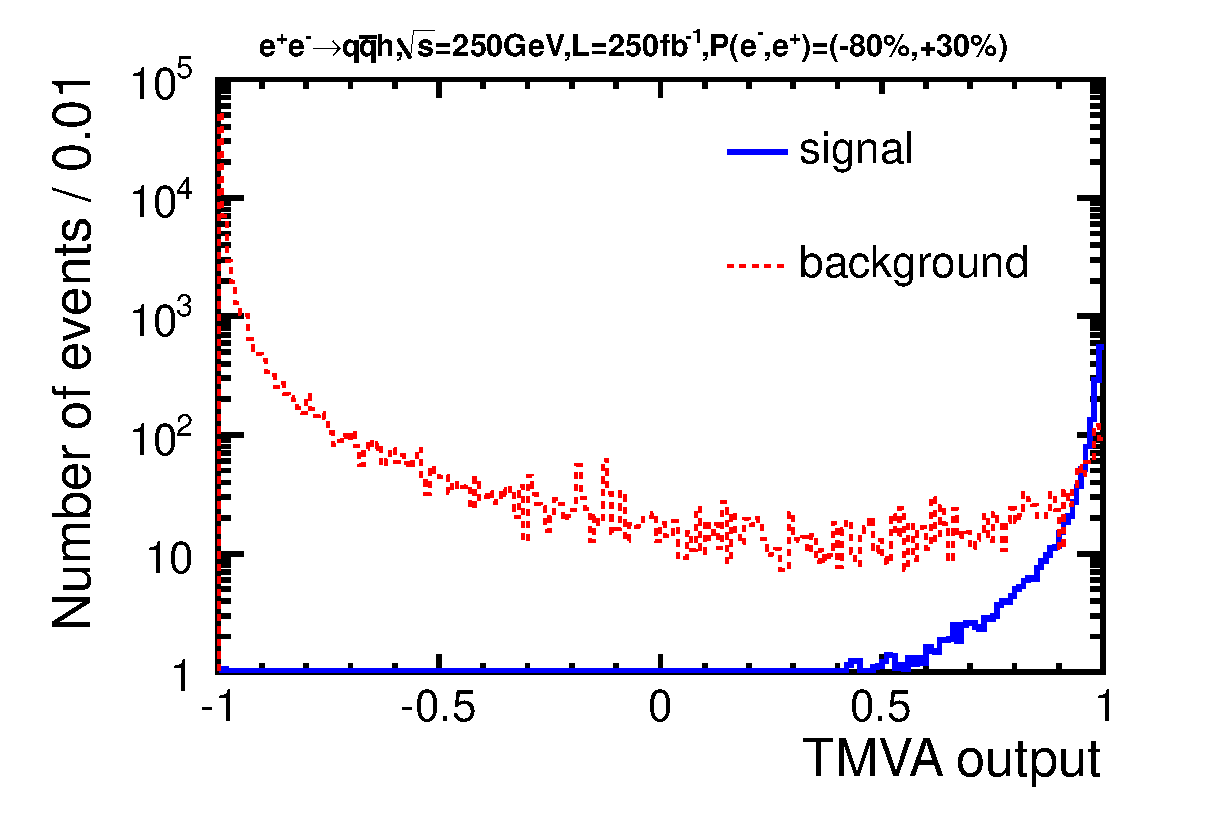
\includegraphics[width=0.85\hsize]{chapters/figures/ZH_qqtautau250_TMVA.eps}
\end{center}
  \caption{MVA output for the signal $e^+e^-\to q\bar{q} h, h\to\tau^+\tau^-$
 and the SM background at 250 GeV \cite{Kawada:2015wea}.}
  \label{fig:qqHtautau250}
\end{figure}

\subsubsection{$\mathrm{BR}(h\to \mathrm{invisible/exotic})$}
\label{sec:higgs:invisible}
As introduced in~\ref{sec:higgs:sigmazh}, the recoil technique enables that 
the Higgs events can be tagged without looking into Higgs decay products. 
This feature is extremely useful for probing Higgs to invisible or other exotic decays.
Full simulation studies are performed for $e^+e^-\to Zh$, $h\to\mathrm{invisible}$
using two signal channels $Z\to q\bar{q}$ and $Z\to l^+l^-$; 
see details in~\cite{Ishikawa:2014,Tian:2015,Kato:2016}. The dominant contribution comes
from $Z\to q\bar{q}$ channel. After all the cuts the remained signal and background events 
are plotted in Fig.\ref{fig:qqHinv250} in the recoil mass spectrum, where the signal
peak would be clearly seen assuming $BR(h\to\mathrm{invisible})=10\%$. 
The main background events come from $ZZ/\nu\bar{\nu}Z\to\nu\bar{\nu}q\bar{q}$ 
and $WW\to qql\nu$.
The estimate of 95\% C.L. upper limit for $BR(h\to invisible)$
is 0.86\% for the left-handed beam polarizations, shown in Table~\ref{tab:higgserrors}. 
A factor of 1.5 lower upper limit can be obtained for the right-handed beam polarizations,
thanks to the much reduced background level.

Other exotic decays have not been studied based on full simulation. Nevertheless
according to the fast simulation in~\cite{Liu:2016zki}, at ILC250 we would be able 
to probe exotic decays with branching ratios of $10^{-3}$ or below.

\begin{figure}
\begin{center}
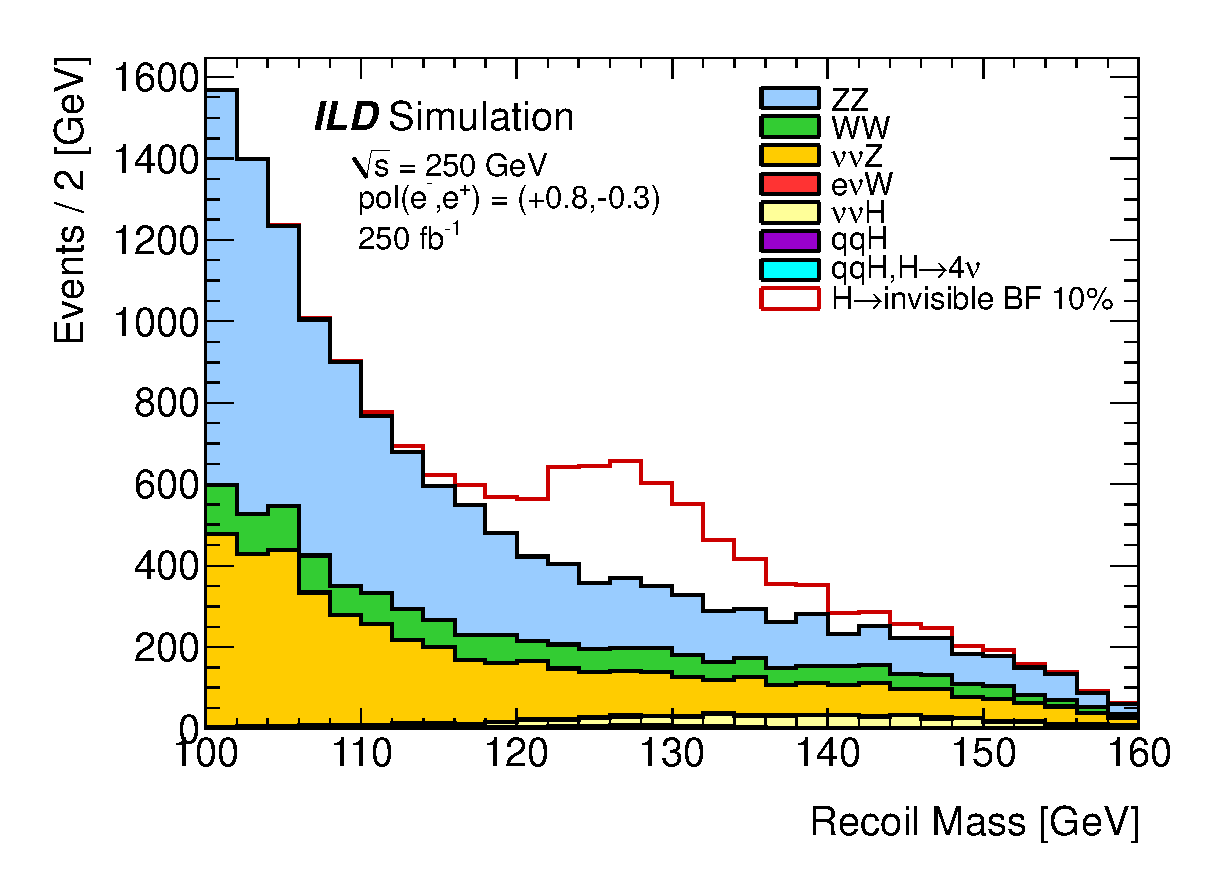
\includegraphics[width=0.85\hsize]{chapters/figures/ZH_qqinv250_right.eps}
\end{center}
  \caption{Recoil mass spectrum against
 $Z\to q\bar{q}$ for signal events $e^+e^-\to Zh, h\to invisible$ assuming $BR(h\to invisible)=10\%$
  and SM background events at 250 GeV for the right-handed beam polarization \cite{Ishikawa:2014}.}
  \label{fig:qqHinv250}
\end{figure}

\subsubsection{$\mathrm{BR}(h\to \mu^+\mu^- / \gamma\gamma / \gamma Z)$}
The measurement of the SM rare decay branching ratios
$\mathrm{BR}(h\to \mu^+\mu^- / \gamma\gamma / \gamma Z)$
are a bit challenging at the ILC, mainly due to the limited number of signal events. 
We expect significant contributions from HL-LHC for these measurements.
Full simulations are performed in~\cite{Kawada:2018wyz,Calancha:2013}, 
and the estimates of statistical uncertainties for
$\sigma_{Zh}\cdot BR_{\mu\mu}$ and $\sigma_{Zh}\cdot BR_{\gamma\gamma}$
are respectively 72\% and 34\%, shown in Table~\ref{tab:higgserrors}. 
$BR(h\to\gamma Z)$ is also studied based on full simulation~\cite{Fujii:2018}, 
a significance of 2$\sigma$ would be expected with full ILC250.

\subsubsection{Higgs CP Properties}
\label{subsubsec:higgstautauCP}
Higgs CP properties can be measured via the
$h\tau\tau$ coupling at the tree level, 
\beq
\Delta{\cal L}_{h\tau\tau}=-\frac{\kappa_\tau y_\tau}{\sqrt{2}}h{\tau^+}
(\cos\Psi_{CP}+i\sin\Psi_{CP}\gamma_5)\tau^-,
\eeq{eqn:CPHtautau}
where the CP phase angle $\Psi_{CP}$ is determined using the transverse spin
correlation between the two $\tau$, as shown in Fig.~\ref{fig:qqHtautauCP} (upper)
in the $\Delta\phi$ (angle between transverse spins of two $\tau$)
distribution for different values of $\Psi_{CP}$. 
The spin of each $\tau$ is estimated using
the polarimeter vector which can be fully reconstructed in some of $\tau$ decay modes,
such as $\tau\to\pi\nu/\rho\nu$,
taking advantage of precise measurements for impact parameters; see the method detail
in~\cite{Jeans:2015vaa}. Full simulation studies are performed using signal channels 
$Z\to q\bar{q}/l^+l^-$ and $h\to \tau^+\tau^-$ in~\cite{Jeans:2018anq}. 
Figure~\ref{fig:qqHtautauCP} shows the distribution of reconstructed $\Delta\phi$
for the remained signal and background events in one of the golden event categories. 
The estimate of statistical uncertainties for CP phase angle is $4.3^\circ$ with full ILC250.
Note that the Higgs CP violating effects can also be probed in $hZZ$ coupling using the
$\tilde{b}$ parameter shown in next section.

\begin{figure}
\begin{tabular}[c]{c}
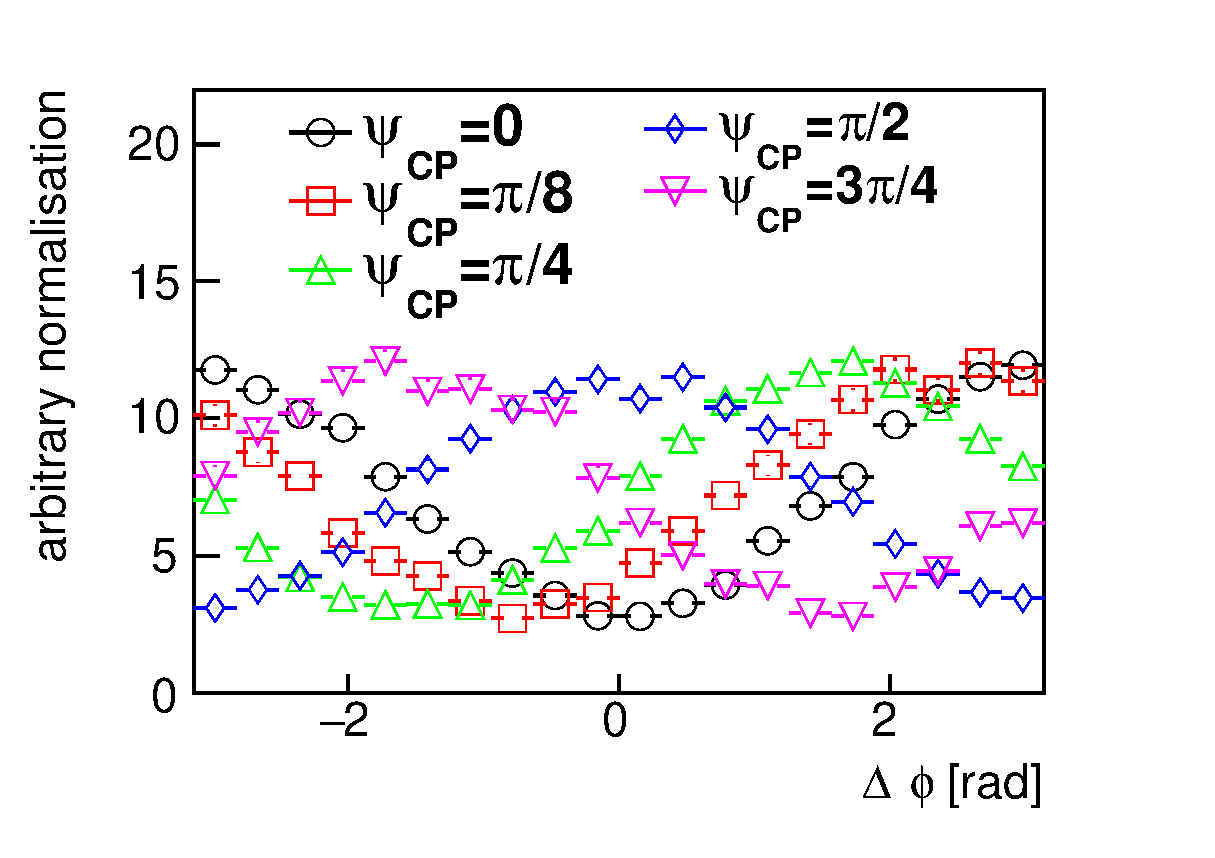
\includegraphics[width=0.85\hsize]{chapters/figures/ZH_qqtautau250_CP1.eps} \\
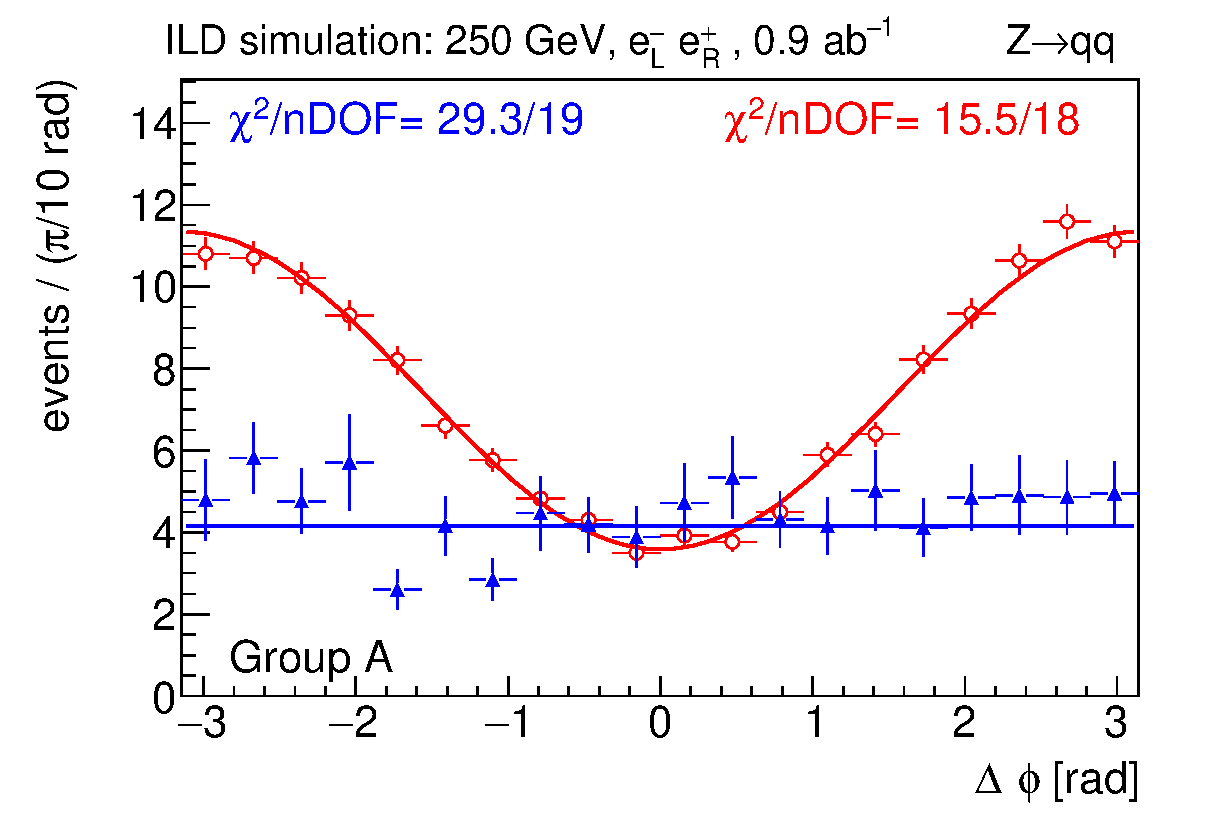
\includegraphics[width=0.85\hsize]{chapters/figures/ZH_qqtautau250_CP2.eps}
\end{tabular}
  \caption{Upper: $\Delta\phi$ distributions at MC Truth level for different 
  values of $\Psi_{CP}$ for the signal $e^+e^-\to q\bar{q} h, h\to\tau^+\tau^-$ at 250 GeV;
  Lower: reconstructed $\Delta\phi$ distributions after all cuts in the dominant category
  for the SM signal (in red) and the SM background (blue) respectively \cite{Jeans:2018anq}.}
  \label{fig:qqHtautauCP}
\end{figure}


\subsubsection{Angular Analyses for Anomalous $HVV$ Couplings}
The $hZZ$ coupling can be deviated from SM not only in total strength but also
in Lorentz structures, which can be detected by measuring differential cross sections.
Full simulation studies are performed using $e^+e^-\to Zh$ events 
for measuring following effective $hZZ$ couplings:
\beq
\Delta{\cal L}_{hZZ}=(1+a)\frac{m_Z^2}{v}hZ_\mu Z^\mu+
\frac{1}{2}\frac{b}{v}hZ_{\mu\nu}{Z}^{\mu\nu}+
\frac{1}{2}\frac{\tilde{b}}{v}hZ_{\mu\nu}\tilde{Z}^{\mu\nu},
\eeq{eqn:CPHZZ}
where the first $a$-term is a rescaling of SM $hZZ$ coupling, the second $b$-term and 
the third $\tilde{b}$-term represent respectively anomalous CP-even and CP-odd 
$hZZ$ couplings. The total cross section $\sigma_{Zh}$ is sensitive to both $a$ and $b$
parameters, but $b$ is distinguished from $a$ in the differential cross sections; see
Fig.~\ref{fig:ZHanomHVV1} (upper) how $Z$ production angle depends on values of $b$.
$\sigma_{Zh}$ depends on $\tilde{b}$ rather weakly, only quadratically. But the angle 
between $Zh$ production plane and $Z$ decay plane, namely $\Delta\Phi$, is very
sensitive to $\tilde{b}$; see Fig.~\ref{fig:ZHanomHVV1} (lower) for $\Delta\Phi$ distributions for
different values of $\tilde{b}$. The analysis details can be found in~\cite{Ogawa:2017bmg}.
The estimate of statistical uncertainties for $a$ and $b$ are 
0.076 and 0.027 respectively, with a large correlation $\rho=-99.17\%$, 
shown in Table~\ref{tab:higgserrors}. This large correlation can be significantly reduced
by measurements at $\sqrt{s}=500$ GeV, as shown in Fig.~\ref{fig:ZHanomHVV2},
because the effect of $b$-term is momentum dependent.
The CP violating parameter $\tilde{b}$ can be determined with a statistical uncertainty of 
0.004 for the full ILC250, with almost no correlation with $a$ or $b$.
\begin{figure}
\begin{tabular}[c]{c}
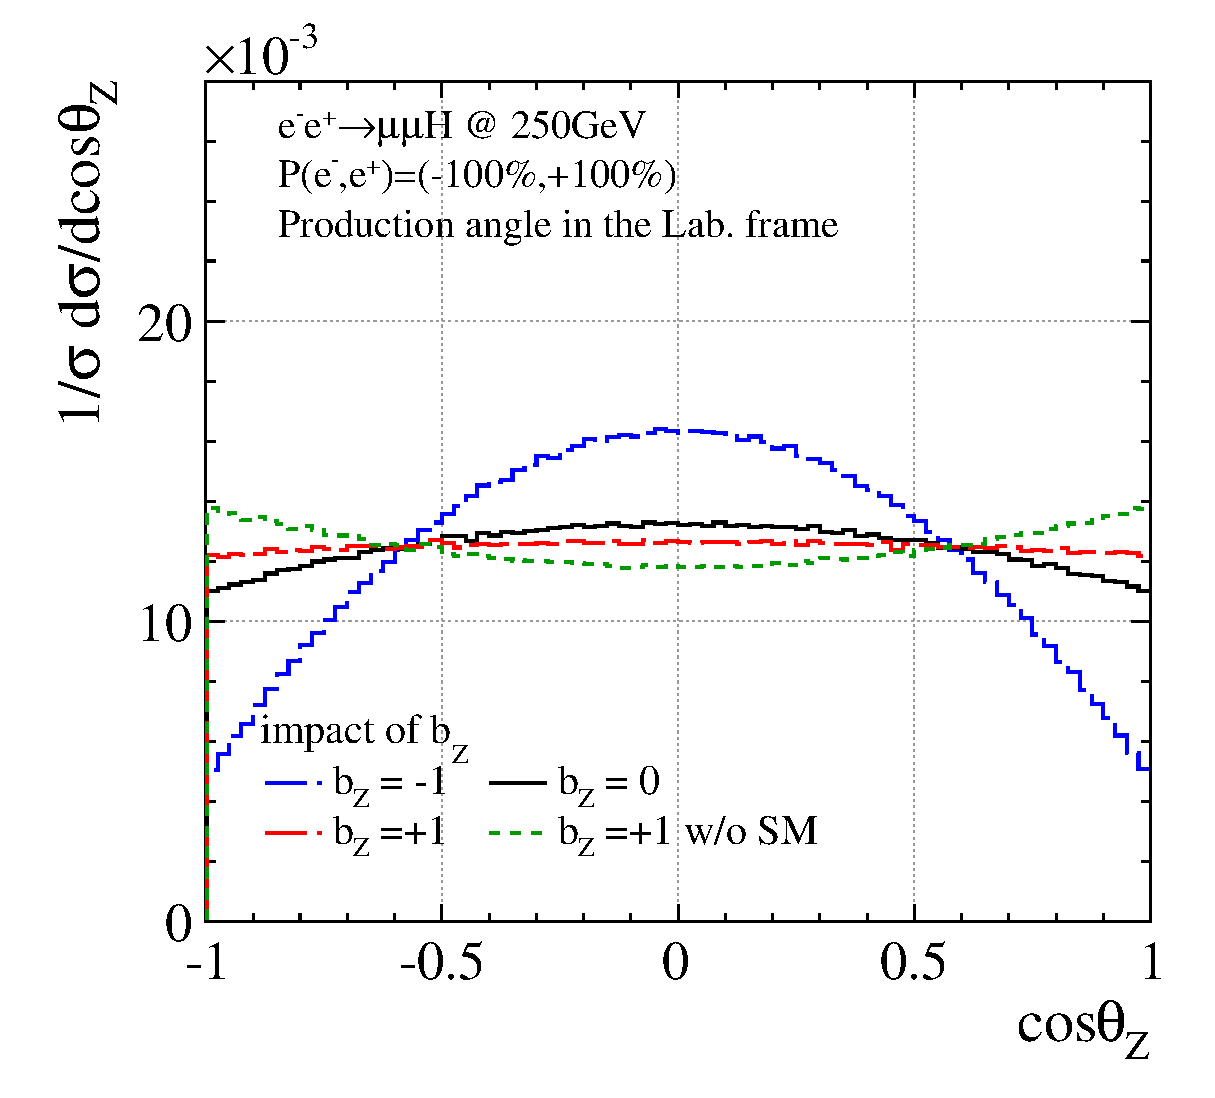
\includegraphics[width=0.85\hsize]{chapters/figures/ZH_anomHVV250_b.eps} \\
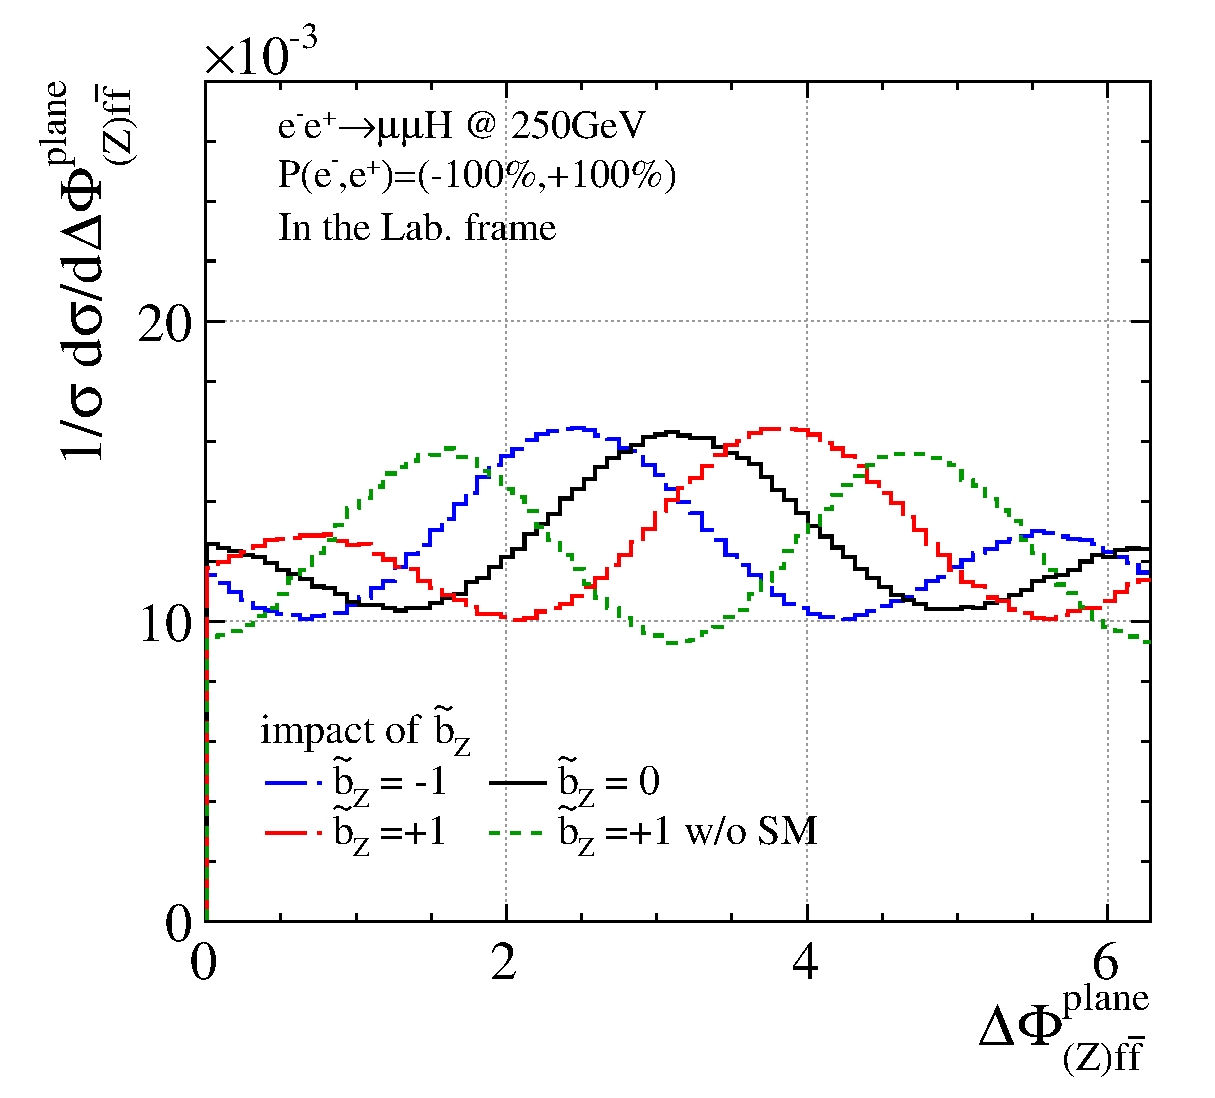
\includegraphics[width=0.85\hsize]{chapters/figures/ZH_anomHVV250_bt.eps} 
\end{tabular}
  \caption{Upper (lower): $\cos\theta_Z$ ($\Delta\Phi$) distributions at MC Truth level for different 
  values of anomalous coupling $b$ ($\tilde{b}$) 
  for the signal $e^+e^-\to \mu^+\mu^- h, h\to everthing$ at 250 GeV;
  \cite{Ogawa:2017bmg}.}
  \label{fig:ZHanomHVV1}
\end{figure}

\begin{figure*}
\begin{center}
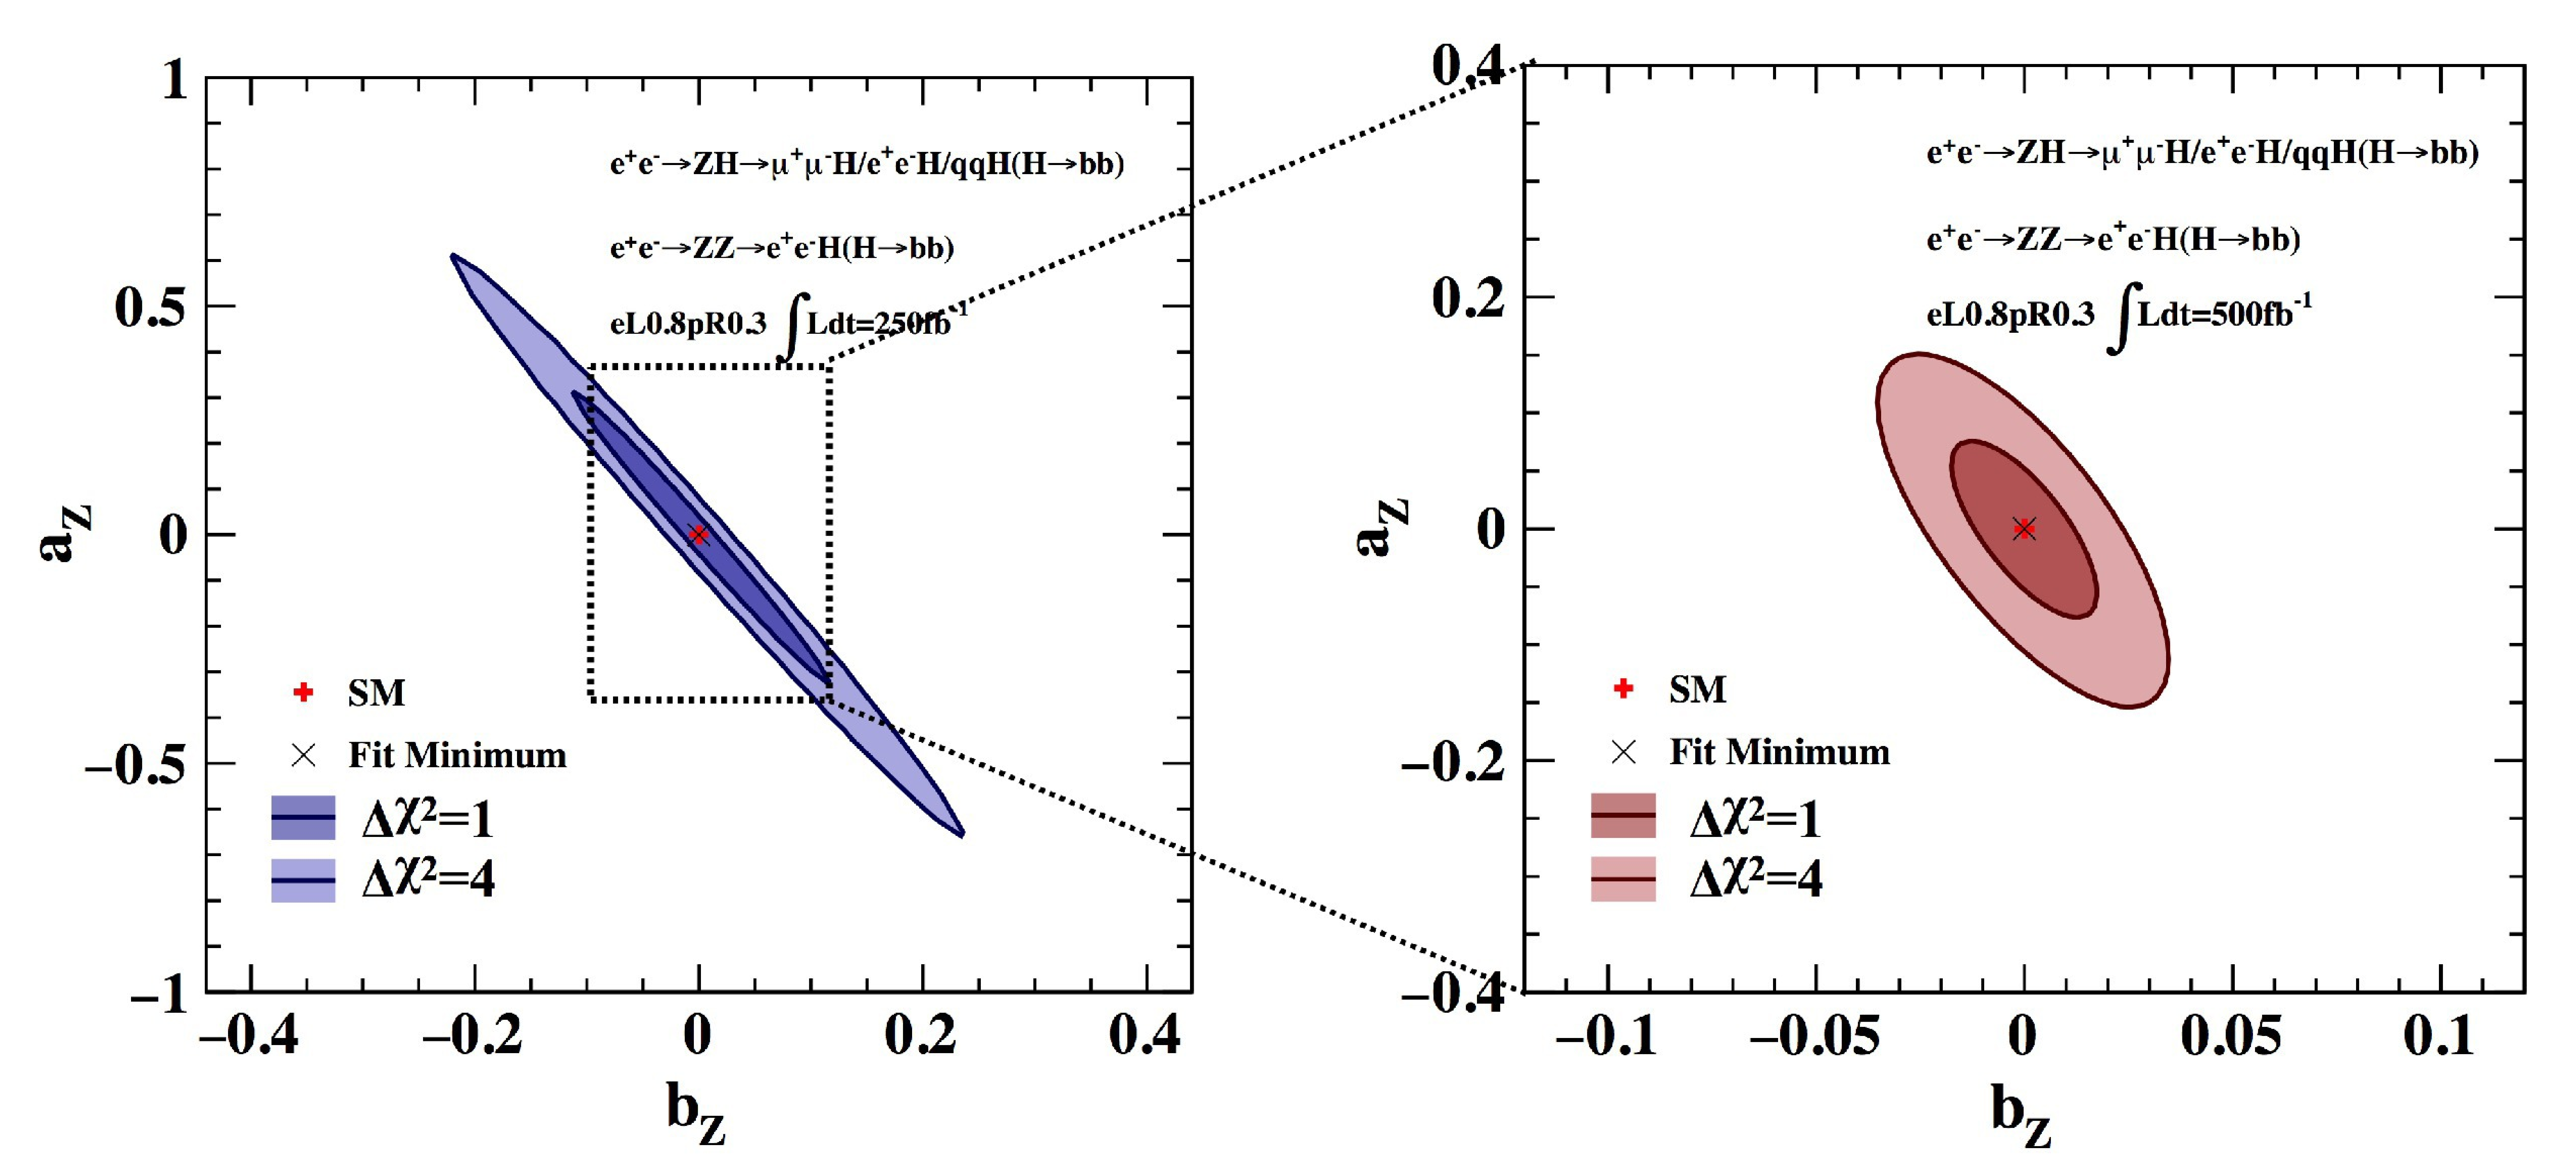
\includegraphics[width=0.85\hsize]{chapters/figures/ZH_anomHVV_ab.eps}
\end{center}
  \caption{68\% and 95\% C.L. contour plots for fitted parameter $a$ versus $b$ at 250 GeV (left)
  and 500 GeV (right) \cite{Ogawa:2017bmg}.}
  \label{fig:ZHanomHVV2}
\end{figure*}
